\subsection{User Interface and Core Functionalities}
\label{sub:ui}

The \gls{UI} is intentionally kept clean for simplicity reasons. \texttt{Bootstrap} is used to provide a consistent look \& feel and responsiveness of the application. As described in \autoref{sub:sassoon:actors} we have three main users in our system which have different abilities\footnote{Abilities are access rights, that are specified via an \texttt{Ability} class that is used by \texttt{cancancan} to provide diversified access-rights to different user groups in our system.} influencing the appearance of the \gls{UI} (eg. a clinician will not be able to create, alter or delete any research questions, however the clinician will still be able to see them as depicted in \autoref{fig:ui:rq}). This approach allows us to use the same \gls{UI}-components for different users without writing them once again (\gls{DRY} principle).



To provide easier access to the underlying \gls{SKB}, research questions and models include a visual representation of their relations as a graph (see \autoref{fig:ui:model}). The system offers four different types of assumptions which have special functionalities (explanation of each type can be found in \autoref{sub:db}).




\begin{figure}[hbtp]
\centering
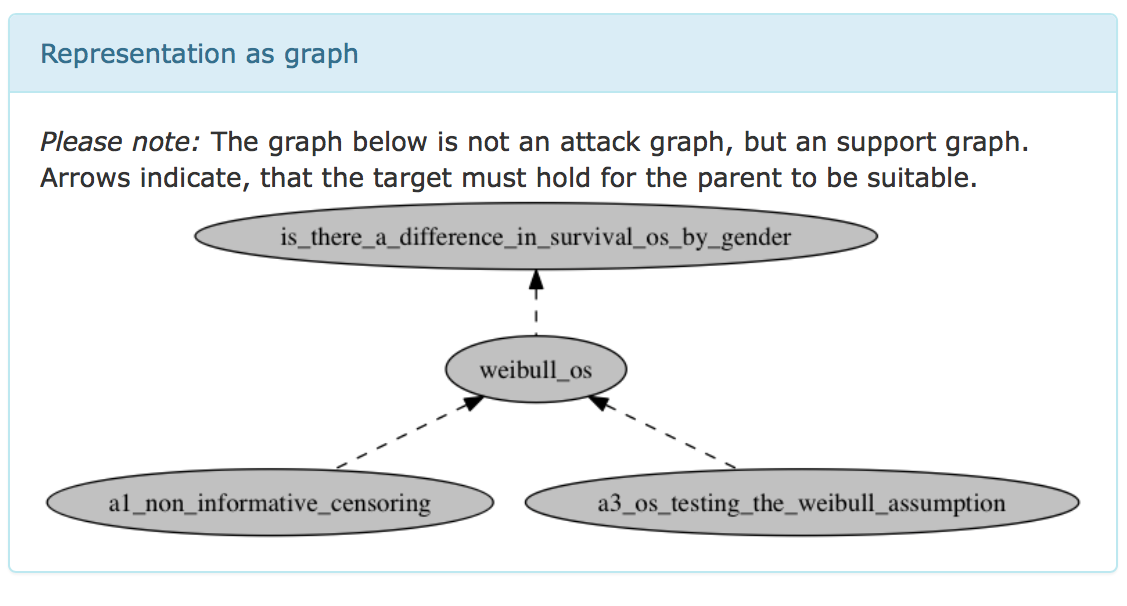
\includegraphics[width=0.6\textwidth]{figures/ui_Weibull_Model}
\caption{Overview over a model as a graph representation, in this particular case the \textit{Weibull model}, which requires two assumptions to hold.}
\label{fig:ui:model}
\end{figure}

Each of those require different attributes which results in different forms during the creation process of new assumptions. For a model to be possible during an analysis, all assumptions assigned to this model need to hold (evaluate to true) regardless of its type. In a second step, the defined \glspl{preference} are evaluated. To do so, all possible models are added to an \gls{EAF} attacking each other as described in \autoref{sub:preferences} and the \glspl{CD} are then added iteratively. This process can be seen in \autoref{fig:analysis:eaf}.

\begin{figure}[htb]
	\centering
	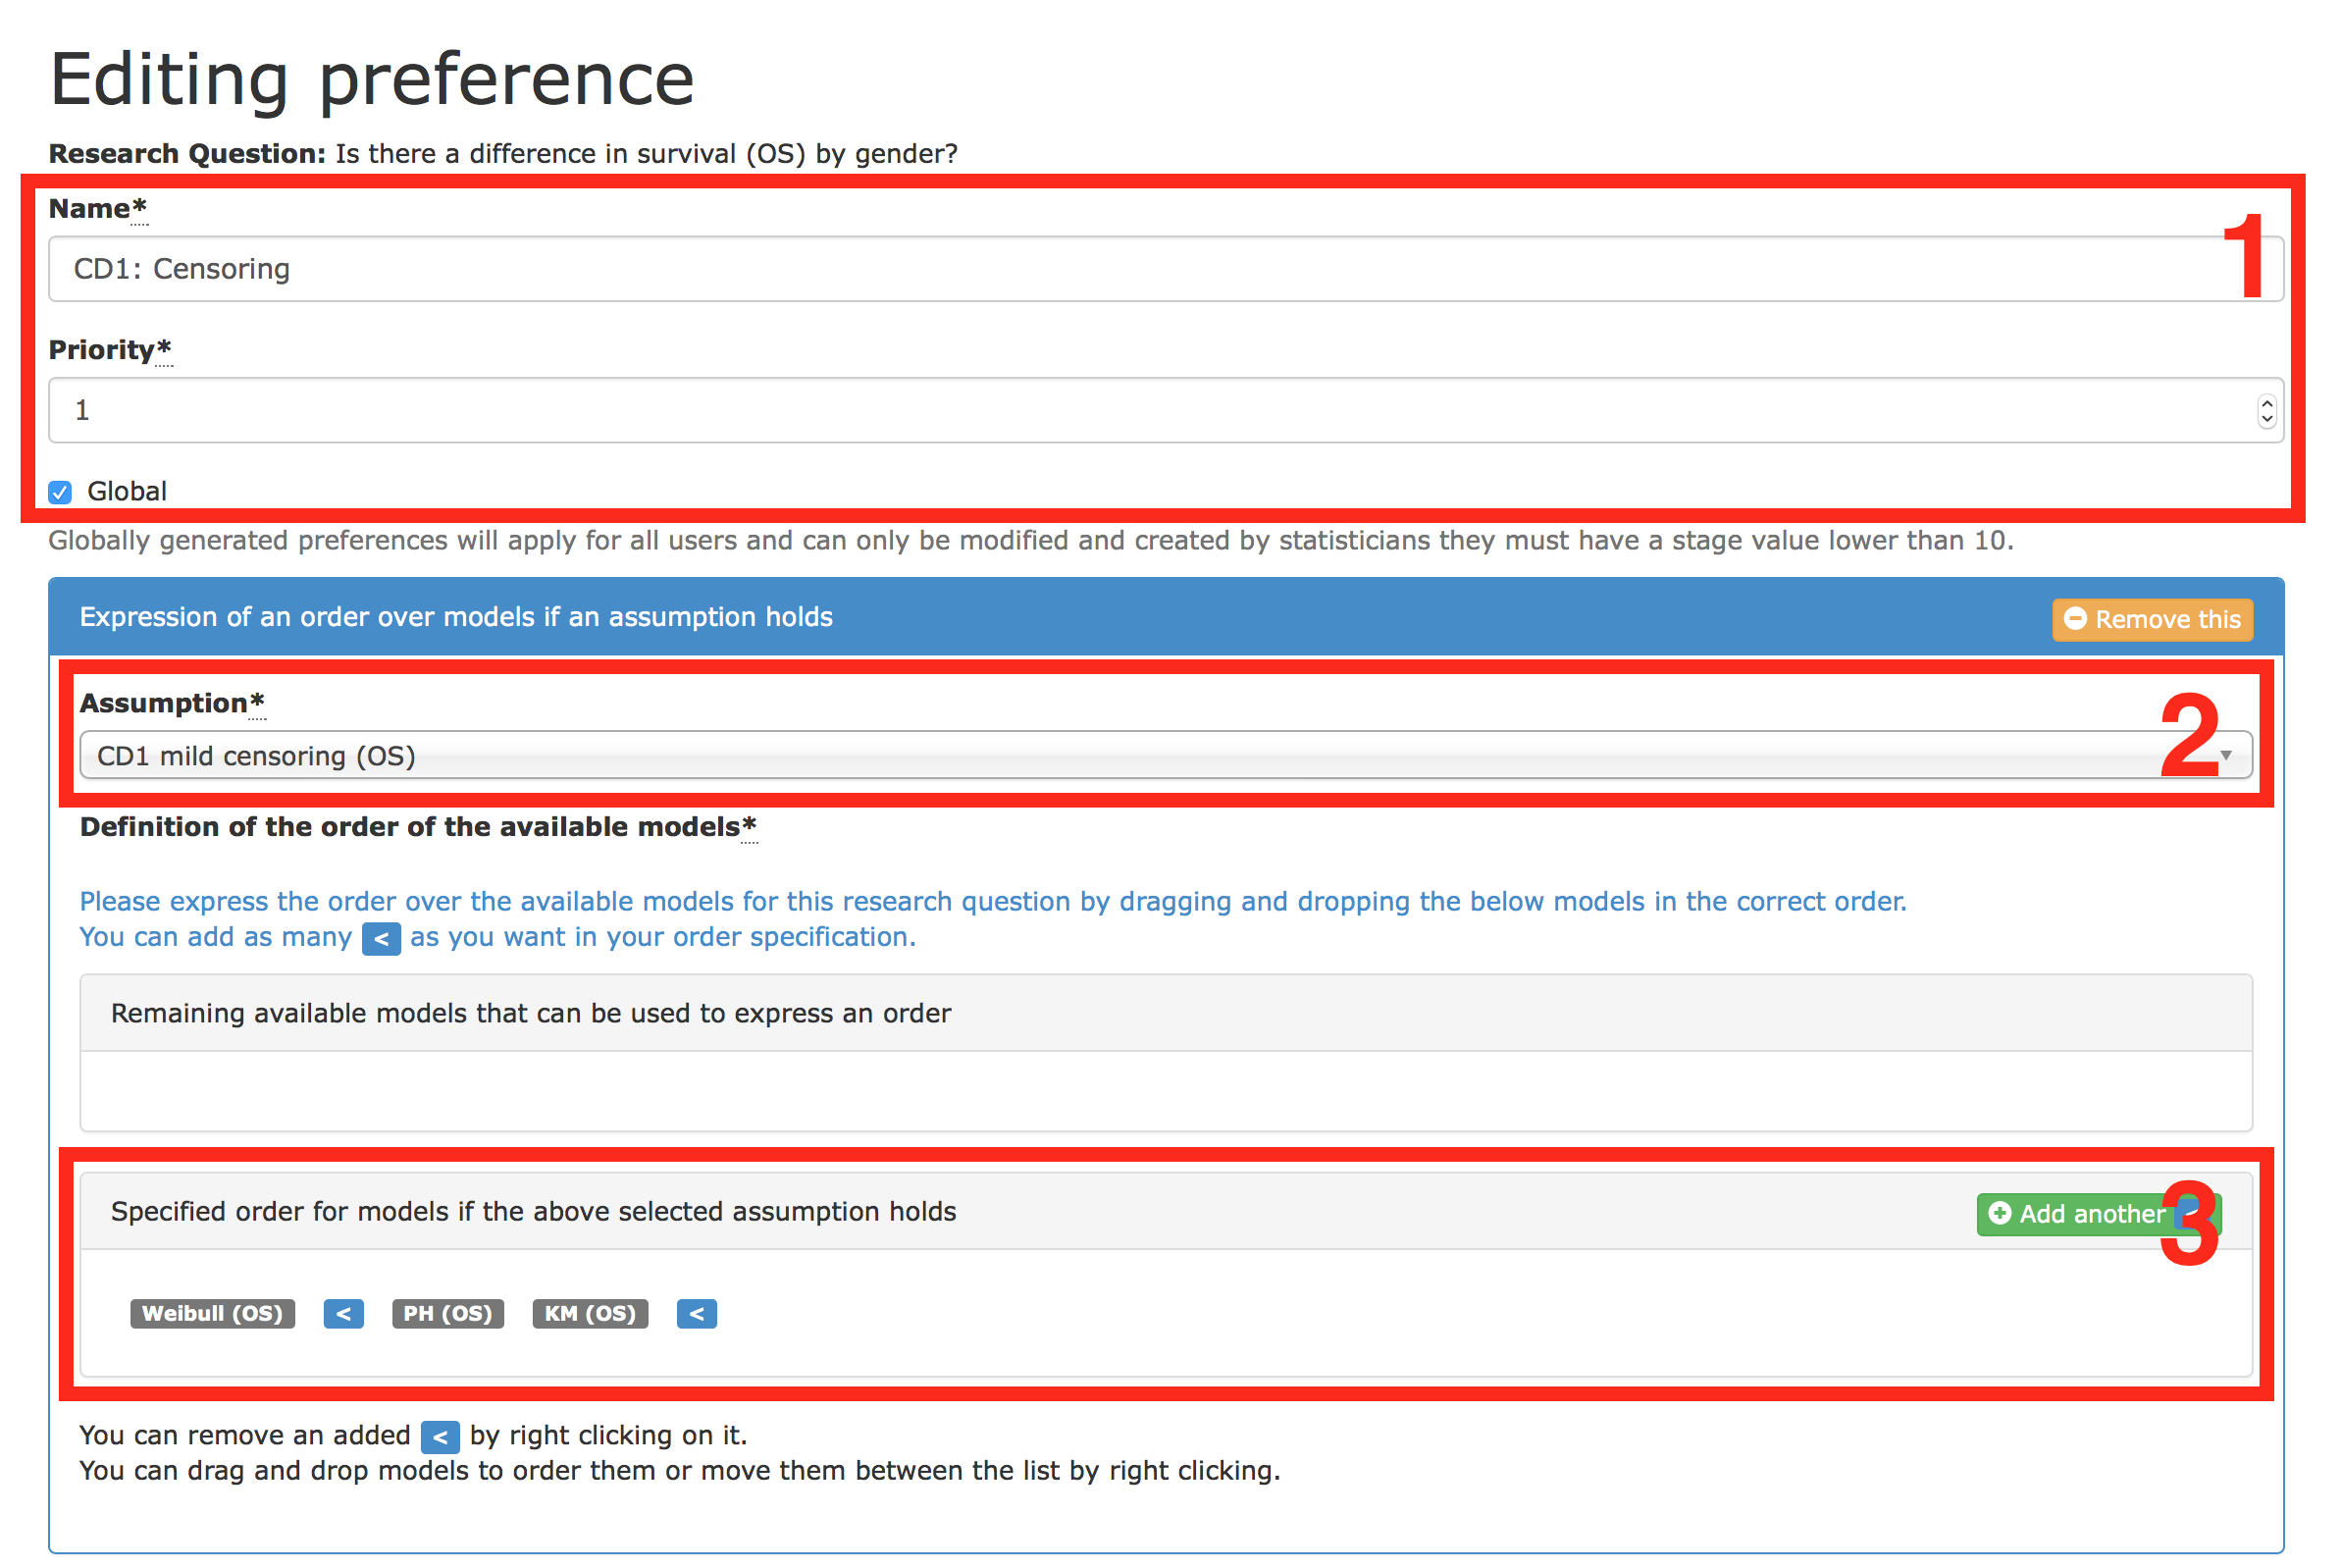
\includegraphics[width=\textwidth]{figures/ui_preference}
	\caption{\gls{UI} to enter preferences between models: General information about this preference including the applicable research question (1), the context under which this preference applies can be defined as assumption (2), and the actual order of the models can be interactively arranged per drag \& drop (3).}
	\label{fig:ui:preference}
\end{figure}


The most complex component from an \gls{UI} perspective are preferences, as they involve context domains and there required assumptions and relative orders per context domain. \autoref{fig:ui:preference} shows how this has been solved: (1) allows the user to enter general details for a preference (availability to users, priority and name). 

For each available context domain for this particular preference, an assumption (2) has to be chosen. A context domain will be applied, if and only if this assumption holds. The relatively order between models can be specified easily via drag \& drop (3). 

This order will be taken into account when analysing the \gls{EAF} at the final step of the analysis process. If a preference is not defined over all available models for a particular research question the performance measurement for this model is undefined and it will stay untouched.

As expressed earlier before, the priority of a preference can be set and defines the order of applying different \glspl{CD}. This ensures, that a clinicians preference will always be less important than the statistical reasons a statistician has entered into the system ensuring reliability and statistical correctness while applying the preferences on possible models.

